\section{Multi-Level 2D Haar Transform}
\subsection{Implimentation}
After performing the Haar transform, one can notice that the "LoLo" section of the transform is largely similar to the original image. As such some gains can be achieved by applying the Haar transform recursively to the LoLo section of the transform. The $n$-point Haar Transform is then defined by recursively applying the Haar Transform to the LoLo section of the level 1 transform $n-1$ times. The implementation is shown below.
\lstinputlisting[language=Octave]{../calcHaar.m}

\subsection{RD curves for Level 1-5 Haar Transform}
Shown below in Figure \ref{fig:RDMultipleHaar} we can see the RD curves for the $Q_{step}$ values mentioned before.

\begin{figure}[!h]
    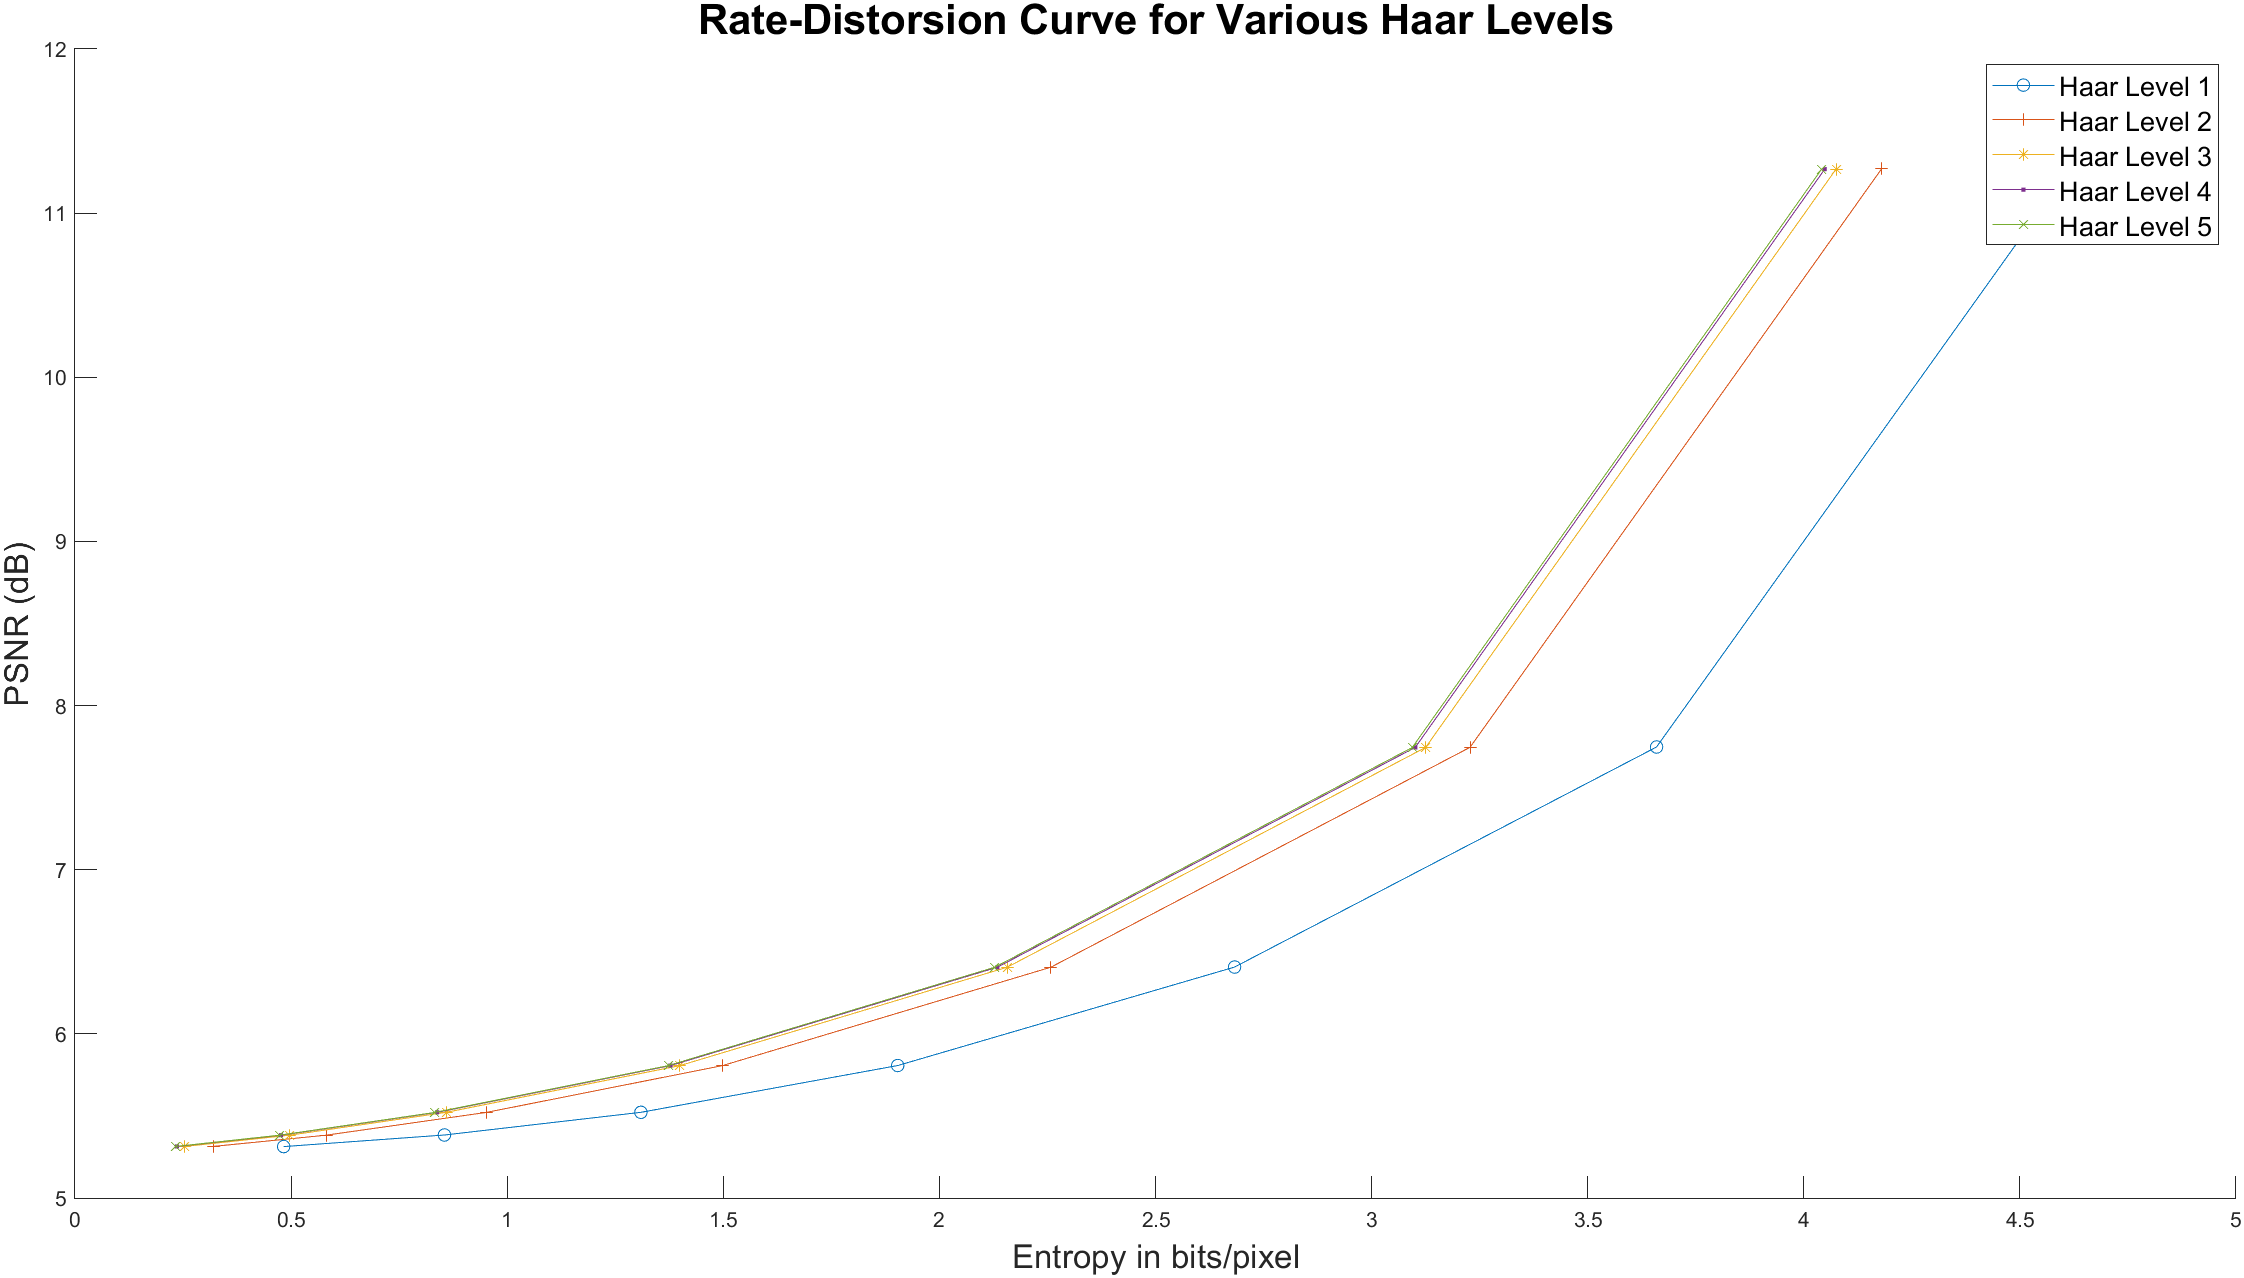
\includegraphics[width=1\textwidth]{RDMultipleHaar.png}
    \centering
    \caption{RD Curve for Multiple Haar Levels}
    \label{fig:RDMultipleHaar}
\end{figure}

\noindent Looking at the curves we see clear diminishing returns as the Haar level increases. Past Haar level 3, the reduction in entropy isn't worth the extra processing time required to calculate it.